\subsubsection{Flöde vid termisk jämvikt}

Vid beräkningen av värmeflödet genom grunden användes geometrin som kan ses i figur \ref{fig:groundheat}. Källaren antas vara belägen en halv meter under marknivån. I samma figur ses även temperaturfördelningen vid termisk jämvikt då markens temperatur långt under huset sätts till konstanta $\unit[8]{^{circ}C}$. Vid markytan sattes konvektionskoefficienten till $h=\unit[15,5]{Wm^{-2}K^{-1}}$, motsvarande en ungefärlig vindhastighet (parallel med ytan) på $\unit[2]{ms^{-1}}$ vid utomhustemperaturen $\unit[0]{^{\circ}C}$. Källarens temperatur antas vara konstant $\unit[10]{^{\circ}C}$ och \textcolor{red}{grundens U-värde approximeras till $\unit[?]{Wm^{-2}K^{-1}}$}.

\begin{figure}
\centering
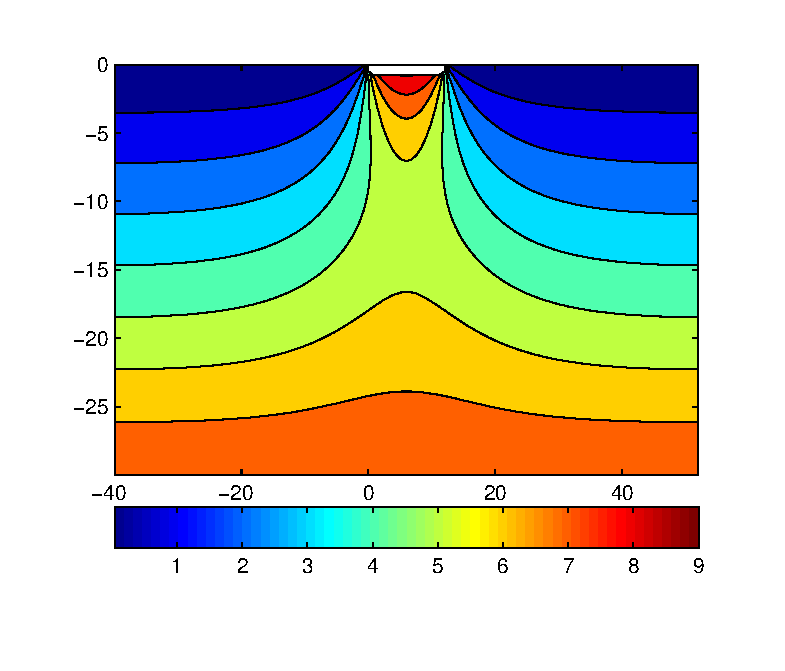
\includegraphics{images/groundheat.eps}
\caption{\label{fig:groundheat}Temperaturen i marken under en byggnad angivet i grader Celsius. Detta är vid termisk jämvikt med statiska temperaturer och temperaturen långt ner i marken satt till konstanta $\unit[8]{^\circ C}$.}
\end{figure}

I figur \ref{fig:groundtemp} kan grundens medeltemperatur som funktion av utomhustemperaturen ses. Med hjälp av dessa värden kan sedan värmeflödena genom grunden beräknas.

\begin{figure}
\centering
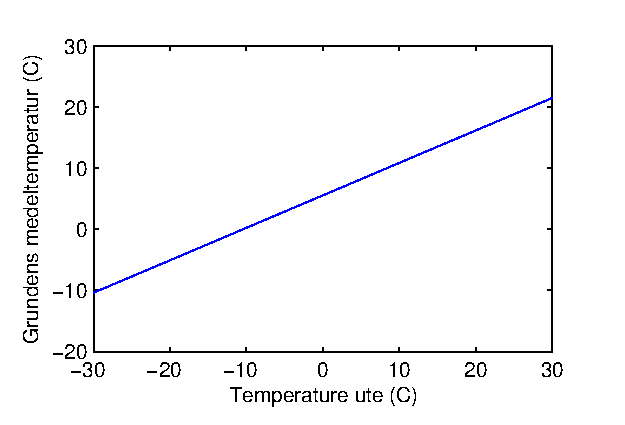
\includegraphics{images/groundtemperature.eps}
\caption{Grundens medeltemperatur mot en referenstemperatur utomhus. Konvektionsparametern är satt till $h = \unit[15,5]{Wm^{-2}K^{-1}}$.}
\label{fig:groundtemp}
\end{figure}
